\section{Quantizing Electric Circuit and the Josephson Junction} \label{appen:LC}
Throughout the project, I mentioned several times that the physical implementation of the qubit is not  the subject of the project and ignored it. It would be a crime no to at least give a simple explanation of the implementation of the qubit, especially since we dedicated and entire section  (section \ref{sec:DRAG}) to the problem with our physical implementation. In this appendix I will try to give a simple explanation of  the qubit as a quantum LC circuit, using the  tools we got when we quantized the electromagnetic field.

This appendix is here for two reasons. The first we already mentioned, to gain some insights on how the qubit is implemented physically. The second, less obvious reason, is to really drive home the point that Dirac's method for Canonical quantization can be applied to any oscillating phenomena. From mechanical oscillator, to the electromagnetic field and even an LC circuit, as we'll see shortly.

\subsection{Quantizing the LC Circuit}
The LC circuit is constructed by connecting a capacitor with capacitance $C$ to a coil with inductance $L$, hence the name, \textit{LC}. Drawing it in a diagram is as shown
\begin{figure}[H]
    \centering
    % TODO: Change image to one with marking of the magnetic inductance field and the  electric capacitance field
    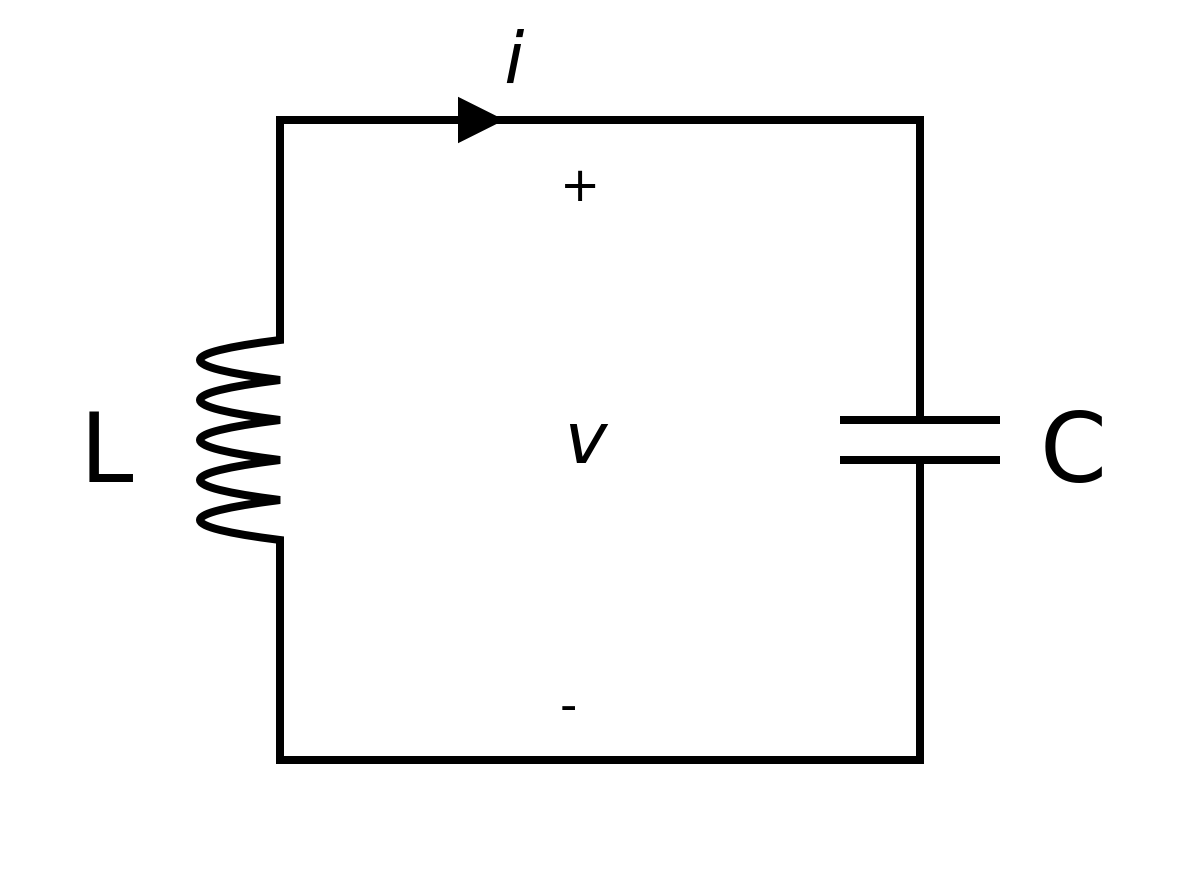
\includegraphics[width=0.4\columnwidth]{LC-circuit.png}
    \caption{The LC circuit} 
    \label{fig:LC-circuit}
\end{figure}

To begin the quantization we first need choose a pair of canonically conjugate variables to represent the state of the system. The most obvious pair of variables would be the voltage $V$ and the current $I$, but turns out they are not canonically conjugate variables. Instead, we'll choose the charge of the capacitor $q$ and the inductor's magnetic flux $\phi$ to be the variables. 

Let's check that they are indeed canonically conjugate. The energy (and therefore, the Hamiltonian) of the capacitor's electric field is given by
\[
    H_C = \frac{q^2}{2C}
\]
and the energy of the magnetic field stored in the inductor is given by
\[
    H_L = \frac{\phi^2}{2L}
\]
Now we can sum these two donations to the Hamiltonian and get that the Hamiltonian of the LC circuit is
\[
    H_{LC}(q, \phi) = \frac{\phi^2}{2L} + \frac{q^2}{2C}
\]
The Hamilton equations in terms of $q$ and $\phi$ are
\begin{align}
    &\dot{q} = \quad \frac{\partial H_{LC}}{\partial \phi} = \quad \frac{\phi}{L} = \quad I \label{eq:def-current}\\
    &\dot{\phi} = -\frac{\partial H_{LC}}{\partial q} = -\frac{q}{C} = -V \label{eq:def-potential}
\end{align}
These equation are correct since \ref{eq:def-current} is the definition of current and \ref{eq:def-potential} is the definition of potential. Therefore $q$ and $\phi$ are canonically conjugate variables and we can go on and quantize them.

To quantize these variables we simply need to replace them with operators
\begin{align*}
    q \rightarrow \hat{q} \\
    \phi \rightarrow \hat{\phi}
\end{align*}
satisfying the commutation relation
\[
    [\hat{q}, \hat{\phi}] = i\hbar
\]
as always with quantum harmonic oscillator we'll define annihilation and creation operators
\begin{align*}
    &\hat{a} = \frac{\hat{q}}{q_0} + i\frac{\hat{\phi}}{\phi_0} \\
    &\hat{a}^\dag = \frac{\hat{q}}{q_0} - i\frac{\hat{\phi}}{\phi_0}
\end{align*}
where
\begin{align*}
    &q_0^2 = 2\hbar\sqrt{\frac{C}{L}} \\
    &\phi_0^2 = 2\hbar\sqrt{\frac{L}{C}}
\end{align*}
% TODO: Maybe don't skip the basic algebra
After some algebra magic we can get the expression of the Hamiltonian
\[
    \hat{H}_{LC} = \hbar \omega (\hat{a}^\dag \hat{a} + \frac{1}{2}) \quad \text{with} \quad \omega = \frac{1}{\sqrt{LC}}
\]
This is the good old expression for the Hamiltonian of a quantum harmonic oscillator and we can treat it as we did with any other quantum harmonic oscillator.

\subsection{Artificial Atoms - The Josephson Effect}
The problem with the simple quantum LC circuit is that it's energy levels are \textit{linear}. By linear, I mean that the difference in energy between two neighboring levels is the same for every level, $E_{n + 1} - E_n = \hbar \omega$ for all $n$\footnote{Unlike an actual atom where the energy difference decreases at higher levels}. This is a problem since we want to treat it as a two level system. If we send a pulse with $\hbar \omega$ energy, we want it to affect only the lower two levels, but since the energy difference between all the levels is the same, sending such a pulse would also excite the higher levels uncontrollably.

We want to introduce \textit{un-linearity} to the levels, so still $E_1 - E_0 = \hbar \omega_{01} $ but $E_2 - E_1 = \hbar \omega_{12}$, $E_3 - E_2 = \hbar \omega_{23}$ and so on, where $\omega_{n\ n+1} \ne \omega_{01}$. This way if the system is only populated at one of the lower two levels and we send a pulse with energy $\hbar \omega$, the only levels affected are the lower two and not the higher ones\footnote{This is obviously an ideal case, as we seen in section \ref{sec:DRAG} with DRAG}.

To create these a-linearities we can use the \textbf{\textit{Josephson Junction}}. A Josephson junction is simply a cut in the wire, a very (very) thin cut, the two pieces of wire are around 10nm apart. The Josephson junction replaces that inductor in the LC circuit. In a circuit diagram it's drawn as a little $x$, and the circuit diagram of the LC circuit with it is
\begin{figure}[H]
    \centering
    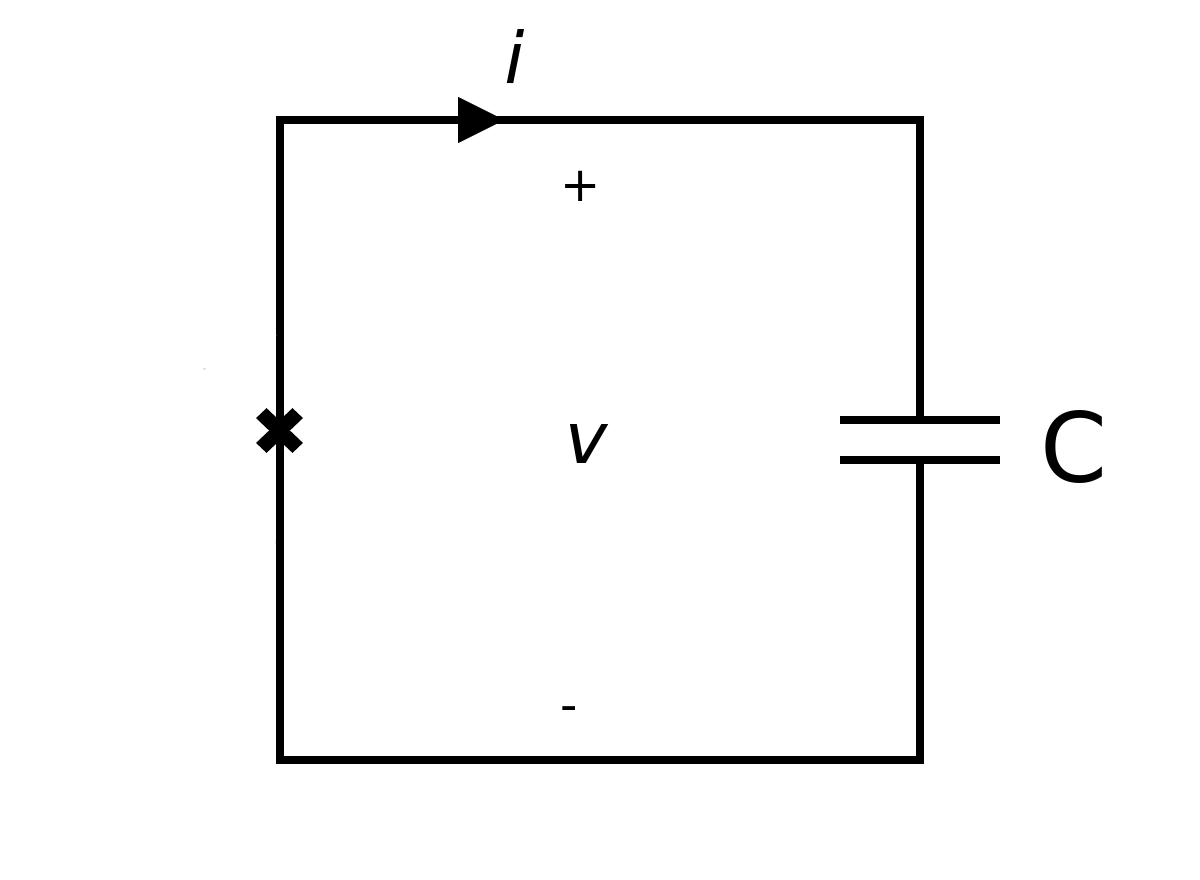
\includegraphics[width=0.43\columnwidth]{LC-circuit-josephson.png}
    \caption{The LC circuit with a Josephson junction} 
    \label{fig:LC-circuit-Josephson}
\end{figure}
And the effect of adding a Josephson junction is replacing the Hamiltonian of the inductor $\frac{\phi^2}{2L}$ with $E_j \cos (\frac{2e}{\hbar} \phi)$.
\[
    \hat{H}_{Josephson} = \frac{\hat{q}^2}{2C} + E_j \cos (\frac{2e}{\hbar} \phi)
\]
This does exactly what we want, for the first level we can approximate the cosine as a parabola and get $E_1 - E_0 = \hbar \omega_{01}$ but since the cosine diverges from the parabola after that the difference between the energy levels lessens and lessens between each pair of higher levels. Here's a visual representation of the energy level of the LC circuit with the Josephson junction
\begin{figure}[H]
    \centering
    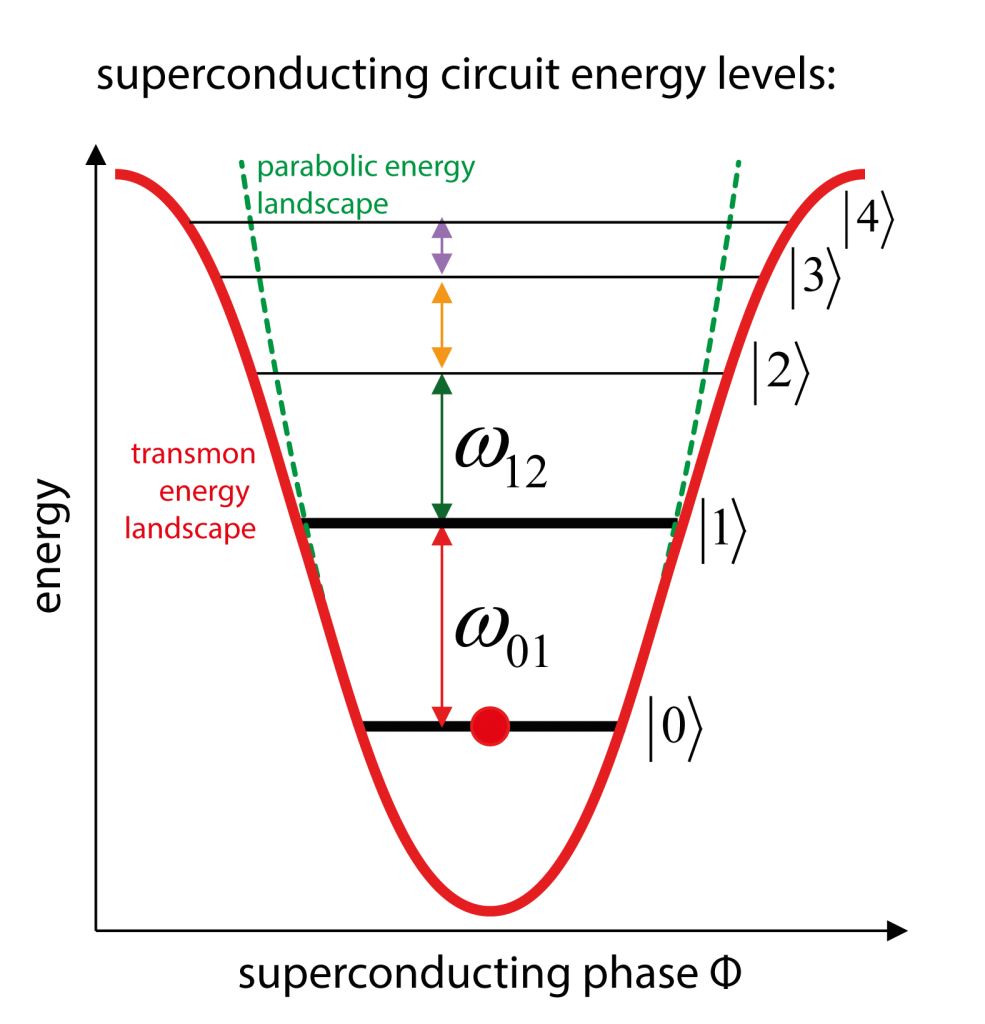
\includegraphics[width=0.4\columnwidth]{josephson-energy-levels.png}
    \caption{Potential of the circuit as a function of the superconducting phase, and the non-linear energy levels of the Josephson junction} 
    \label{fig:Josephson-energy-levels}
\end{figure}
We can treat the Josephson junction as a potential barrier, and calculate the wave function on both sides of the wire.

We'll call the wave function on one side of the junction $\psi_1$ and on the other side $\psi_2$, their dynamics are determined by the coupled shr\"{o}dinger equations:
\begin{align*}
    &i\hbar\frac{\partial \psi_1}{\partial t} = \mu_1 \psi_1 + K \psi_2 \\
    &i\hbar\frac{\partial \psi_2}{\partial t} = \mu_2 \psi_2 + K \psi_1 
\end{align*}
Where $K$ is the coupling across the barrier and $\mu_{1/2}$ are the lowest energy states of each wave function. We'll "guess" solutions of the form
\[
    \psi_{1/2} = \sqrt{n_{1/2}}e^{i\theta_{1/2}}
\]
Yielding the two equations
\begin{align*}
    &\hbar \frac{\partial n_1}{\partial t} = - \hbar \frac{\partial n_2}{\partial t} = 2K \sqrt{n_1 n_2} \sin (\theta_2 - \theta_1) \\
    -&\hbar \frac{\partial (\theta_2 - \theta_1)}{\partial t} = \mu_2 - \mu_1
\end{align*}
$n_{1/2}$ are the density of cooper pairs, and by definition of the current, the current is $\frac{\partial n_1}{\partial t}$. When voltage is applied the energy levels shift as $\mu_2 - \mu_1 = 2eV$. Finally to make the equations shorter we'll write $I_0 = 2K\sqrt{n_1 n_2}$ and $\delta = \theta_2 - \theta_1$. The equations now become
\begin{align*}
    &I = I_0 \sin \delta \\
    &\frac{\partial \delta}{\partial t} = \frac{2eV}{\hbar}
\end{align*}

We can now calculate the electric power (which is the derivative of the energy) from the classical equation
\[
    \frac{\partial E}{\partial t} = P = I V = (I_0 \sin \delta) \cdot (\frac{\hbar}{2e} \frac{\partial \delta}{\partial t}) = -\frac{I_0 \hbar}{2e} \frac{\partial \cos \delta}{\partial t}
\]
Integrating over time, we get that the expression for the energy is
\[
    E = -\frac{I_0 \hbar}{2e} \cos \delta
\]
If we define $E_j = -\frac{I_0 \hbar}{2e}$, replace $\delta$ with $\hat{\phi}$, and replace the energy with the Hamiltonian, we get
\[
    \hat{H}_{Josephson} = E_j \cos \hat{\phi}
\]
just as we've written earlier.

This is not the best treatment of the Josephson junction but it's a rough idea of the explanation. This expression gives us the a-linearities we want to get to implement the qubit.